\documentclass[twoside]{book}

% Packages required by doxygen
\usepackage{fixltx2e}
\usepackage{calc}
\usepackage{doxygen}
\usepackage[export]{adjustbox} % also loads graphicx
\usepackage{graphicx}
\usepackage[utf8]{inputenc}
\usepackage{makeidx}
\usepackage{multicol}
\usepackage{multirow}
\PassOptionsToPackage{warn}{textcomp}
\usepackage{textcomp}
\usepackage[nointegrals]{wasysym}
\usepackage[table]{xcolor}

% Font selection
\usepackage[T1]{fontenc}
\usepackage[scaled=.90]{helvet}
\usepackage{courier}
\usepackage{amssymb}
\usepackage{sectsty}
\renewcommand{\familydefault}{\sfdefault}
\allsectionsfont{%
  \fontseries{bc}\selectfont%
  \color{darkgray}%
}
\renewcommand{\DoxyLabelFont}{%
  \fontseries{bc}\selectfont%
  \color{darkgray}%
}
\newcommand{\+}{\discretionary{\mbox{\scriptsize$\hookleftarrow$}}{}{}}

% Page & text layout
\usepackage{geometry}
\geometry{%
  a4paper,%
  top=2.5cm,%
  bottom=2.5cm,%
  left=2.5cm,%
  right=2.5cm%
}
\tolerance=750
\hfuzz=15pt
\hbadness=750
\setlength{\emergencystretch}{15pt}
\setlength{\parindent}{0cm}
\setlength{\parskip}{3ex plus 2ex minus 2ex}
\makeatletter
\renewcommand{\paragraph}{%
  \@startsection{paragraph}{4}{0ex}{-1.0ex}{1.0ex}{%
    \normalfont\normalsize\bfseries\SS@parafont%
  }%
}
\renewcommand{\subparagraph}{%
  \@startsection{subparagraph}{5}{0ex}{-1.0ex}{1.0ex}{%
    \normalfont\normalsize\bfseries\SS@subparafont%
  }%
}
\makeatother

% Headers & footers
\usepackage{fancyhdr}
\pagestyle{fancyplain}
\fancyhead[LE]{\fancyplain{}{\bfseries\thepage}}
\fancyhead[CE]{\fancyplain{}{}}
\fancyhead[RE]{\fancyplain{}{\bfseries\leftmark}}
\fancyhead[LO]{\fancyplain{}{\bfseries\rightmark}}
\fancyhead[CO]{\fancyplain{}{}}
\fancyhead[RO]{\fancyplain{}{\bfseries\thepage}}
\fancyfoot[LE]{\fancyplain{}{}}
\fancyfoot[CE]{\fancyplain{}{}}
\fancyfoot[RE]{\fancyplain{}{\bfseries\scriptsize Generated by Doxygen }}
\fancyfoot[LO]{\fancyplain{}{\bfseries\scriptsize Generated by Doxygen }}
\fancyfoot[CO]{\fancyplain{}{}}
\fancyfoot[RO]{\fancyplain{}{}}
\renewcommand{\footrulewidth}{0.4pt}
\renewcommand{\chaptermark}[1]{%
  \markboth{#1}{}%
}
\renewcommand{\sectionmark}[1]{%
  \markright{\thesection\ #1}%
}

% Indices & bibliography
\usepackage{natbib}
\usepackage[titles]{tocloft}
\setcounter{tocdepth}{3}
\setcounter{secnumdepth}{5}
\makeindex

% Hyperlinks (required, but should be loaded last)
\usepackage{ifpdf}
\ifpdf
  \usepackage[pdftex,pagebackref=true]{hyperref}
\else
  \usepackage[ps2pdf,pagebackref=true]{hyperref}
\fi
\hypersetup{%
  colorlinks=true,%
  linkcolor=blue,%
  citecolor=blue,%
  unicode%
}

% Custom commands
\newcommand{\clearemptydoublepage}{%
  \newpage{\pagestyle{empty}\cleardoublepage}%
}

\usepackage{caption}
\captionsetup{labelsep=space,justification=centering,font={bf},singlelinecheck=off,skip=4pt,position=top}

%===== C O N T E N T S =====

\begin{document}

% Titlepage & ToC
\hypersetup{pageanchor=false,
             bookmarksnumbered=true,
             pdfencoding=unicode
            }
\pagenumbering{alph}
\begin{titlepage}
\vspace*{7cm}
\begin{center}%
{\Large My Project }\\
\vspace*{1cm}
{\large Generated by Doxygen 1.8.14}\\
\end{center}
\end{titlepage}
\clearemptydoublepage
\pagenumbering{roman}
\tableofcontents
\clearemptydoublepage
\pagenumbering{arabic}
\hypersetup{pageanchor=true}

%--- Begin generated contents ---
\chapter{Namespace Index}
\section{Namespace List}
Here is a list of all documented namespaces with brief descriptions\+:\begin{DoxyCompactList}
\item\contentsline{section}{\mbox{\hyperlink{namespace_linq}{Linq}} }{\pageref{namespace_linq}}{}
\end{DoxyCompactList}

\chapter{Hierarchical Index}
\section{Class Hierarchy}
This inheritance list is sorted roughly, but not completely, alphabetically\+:\begin{DoxyCompactList}
\item \contentsline{section}{Linq.\+Change\+Tracker\+Entry}{\pageref{class_linq_1_1_change_tracker_entry}}{}
\item \contentsline{section}{Linq.\+Expression\+Tree\+Visitor}{\pageref{class_linq_1_1_expression_tree_visitor}}{}
\begin{DoxyCompactList}
\item \contentsline{section}{Linq.\+Post\+Gre\+Sql\+Expression\+Tree\+Visitor}{\pageref{class_linq_1_1_post_gre_sql_expression_tree_visitor}}{}
\end{DoxyCompactList}
\item I\+Change\+Tracker\begin{DoxyCompactList}
\item \contentsline{section}{Linq.\+Change\+Tracker}{\pageref{class_linq_1_1_change_tracker}}{}
\end{DoxyCompactList}
\item I\+Database\begin{DoxyCompactList}
\item \contentsline{section}{Linq.\+Post\+Gre\+Sql\+Database}{\pageref{class_linq_1_1_post_gre_sql_database}}{}
\end{DoxyCompactList}
\item I\+Queryable\begin{DoxyCompactList}
\item \contentsline{section}{Linq.\+Demo\+Linq$<$ T $>$}{\pageref{class_linq_1_1_demo_linq}}{}
\end{DoxyCompactList}
\item \contentsline{section}{Linq.\+Or\+Mapper}{\pageref{class_linq_1_1_or_mapper}}{}
\item \contentsline{section}{Linq.\+Change\+Tracker\+Entry.\+Pair$<$ T1, T2 $>$}{\pageref{class_linq_1_1_change_tracker_entry_1_1_pair}}{}
\item \contentsline{section}{Linq.\+Program}{\pageref{class_linq_1_1_program}}{}
\end{DoxyCompactList}

\chapter{Class Index}
\section{Class List}
Here are the classes, structs, unions and interfaces with brief descriptions\+:\begin{DoxyCompactList}
\item\contentsline{section}{\mbox{\hyperlink{class_linq_1_1_change_tracker}{Linq.\+Change\+Tracker}} }{\pageref{class_linq_1_1_change_tracker}}{}
\item\contentsline{section}{\mbox{\hyperlink{class_linq_1_1_change_tracker_entry}{Linq.\+Change\+Tracker\+Entry}} }{\pageref{class_linq_1_1_change_tracker_entry}}{}
\item\contentsline{section}{\mbox{\hyperlink{class_linq_1_1_demo_linq}{Linq.\+Demo\+Linq$<$ T $>$}} }{\pageref{class_linq_1_1_demo_linq}}{}
\item\contentsline{section}{\mbox{\hyperlink{class_linq_1_1_expression_tree_visitor}{Linq.\+Expression\+Tree\+Visitor}} }{\pageref{class_linq_1_1_expression_tree_visitor}}{}
\item\contentsline{section}{\mbox{\hyperlink{class_linq_1_1_or_mapper}{Linq.\+Or\+Mapper}} }{\pageref{class_linq_1_1_or_mapper}}{}
\item\contentsline{section}{\mbox{\hyperlink{class_linq_1_1_change_tracker_entry_1_1_pair}{Linq.\+Change\+Tracker\+Entry.\+Pair$<$ T1, T2 $>$}} \\*Represents \mbox{\hyperlink{class_linq_1_1_change_tracker_entry_1_1_pair}{Pair}} of Values, that may be changed anytime }{\pageref{class_linq_1_1_change_tracker_entry_1_1_pair}}{}
\item\contentsline{section}{\mbox{\hyperlink{class_linq_1_1_post_gre_sql_database}{Linq.\+Post\+Gre\+Sql\+Database}} }{\pageref{class_linq_1_1_post_gre_sql_database}}{}
\item\contentsline{section}{\mbox{\hyperlink{class_linq_1_1_post_gre_sql_expression_tree_visitor}{Linq.\+Post\+Gre\+Sql\+Expression\+Tree\+Visitor}} }{\pageref{class_linq_1_1_post_gre_sql_expression_tree_visitor}}{}
\item\contentsline{section}{\mbox{\hyperlink{class_linq_1_1_program}{Linq.\+Program}} }{\pageref{class_linq_1_1_program}}{}
\end{DoxyCompactList}

\chapter{Namespace Documentation}
\hypertarget{namespace_linq}{}\section{Linq Namespace Reference}
\label{namespace_linq}\index{Linq@{Linq}}
\subsection*{Classes}
\begin{DoxyCompactItemize}
\item 
class \mbox{\hyperlink{class_linq_1_1_change_tracker}{Change\+Tracker}}
\item 
class \mbox{\hyperlink{class_linq_1_1_change_tracker_entry}{Change\+Tracker\+Entry}}
\item 
class \mbox{\hyperlink{class_linq_1_1_demo_linq}{Demo\+Linq}}
\item 
class {\bfseries Demo\+Linq\+Provider}
\item 
class \mbox{\hyperlink{class_linq_1_1_expression_tree_visitor}{Expression\+Tree\+Visitor}}
\item 
class \mbox{\hyperlink{class_linq_1_1_or_mapper}{Or\+Mapper}}
\item 
class \mbox{\hyperlink{class_linq_1_1_post_gre_sql_database}{Post\+Gre\+Sql\+Database}}
\item 
class \mbox{\hyperlink{class_linq_1_1_post_gre_sql_expression_tree_visitor}{Post\+Gre\+Sql\+Expression\+Tree\+Visitor}}
\item 
class \mbox{\hyperlink{class_linq_1_1_program}{Program}}
\end{DoxyCompactItemize}

\chapter{Class Documentation}
\hypertarget{class_linq_1_1_change_tracker}{}\section{Linq.\+Change\+Tracker Class Reference}
\label{class_linq_1_1_change_tracker}\index{Linq.\+Change\+Tracker@{Linq.\+Change\+Tracker}}
Inheritance diagram for Linq.\+Change\+Tracker\+:\begin{figure}[H]
\begin{center}
\leavevmode
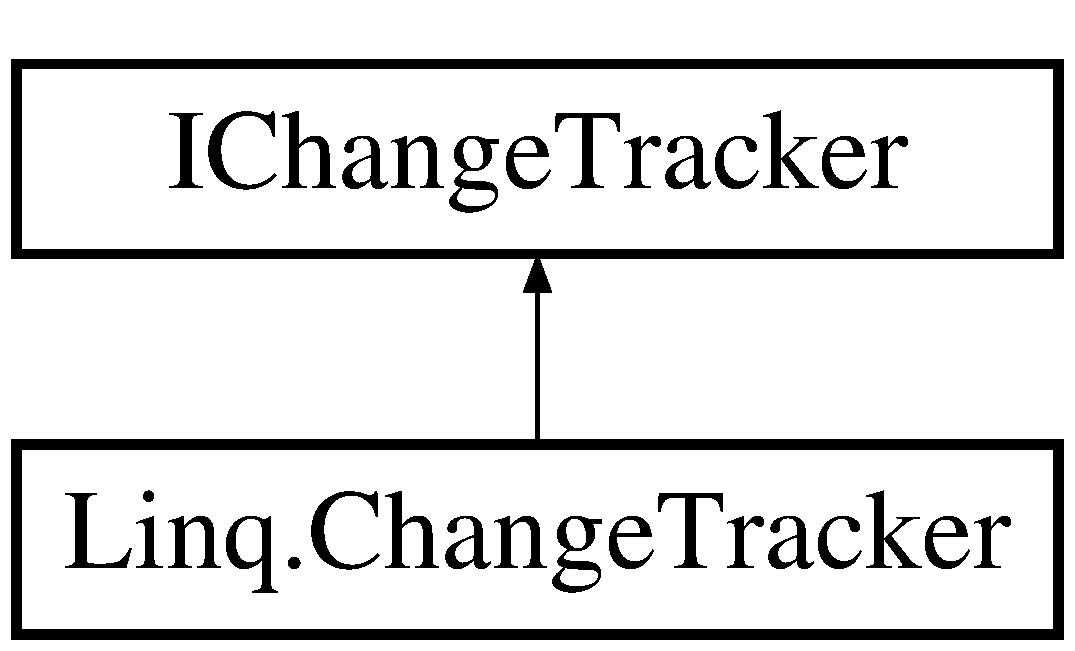
\includegraphics[height=2.000000cm]{class_linq_1_1_change_tracker}
\end{center}
\end{figure}
\subsection*{Public Member Functions}
\begin{DoxyCompactItemize}
\item 
List$<$ \mbox{\hyperlink{class_linq_1_1_change_tracker_entry}{Change\+Tracker\+Entry}} $>$ \mbox{\hyperlink{class_linq_1_1_change_tracker_a2e57cf68dc70deca33a3a9e5e7aa9184}{Detect\+Changes}} ()
\begin{DoxyCompactList}\small\item\em Detects Objects that have been modified, added, or deleted and compiles them into a new List Compute\+Changes should be called after this \end{DoxyCompactList}\item 
void \mbox{\hyperlink{class_linq_1_1_change_tracker_aa53380f4a4352608f221ea918815d7c1}{Insert}} (object obj)
\begin{DoxyCompactList}\small\item\em Inserts an object to be tracked \end{DoxyCompactList}\item 
void \mbox{\hyperlink{class_linq_1_1_change_tracker_a6d14dc387040af11f769e348a98e77f9}{Delete}} (object obj)
\begin{DoxyCompactList}\small\item\em Marks an object as deleted, but doesn\textquotesingle{}t delete the object itself \end{DoxyCompactList}\item 
void \mbox{\hyperlink{class_linq_1_1_change_tracker_ab0d470a3095ae5a0a7ae80fbfdcf614b}{Track}} (object obj)
\begin{DoxyCompactList}\small\item\em Inserts an object into the List of tracked objects and marks it as unmodified \end{DoxyCompactList}\item 
void \mbox{\hyperlink{class_linq_1_1_change_tracker_a8274e4dca2ddc943c748deaca6e6a0a0}{Compute\+Changes}} ()
\begin{DoxyCompactList}\small\item\em resolves the status to delete deleted objects, and update the other ones. \end{DoxyCompactList}\item 
\mbox{\Hypertarget{class_linq_1_1_change_tracker_a45301c9a0a9e32e1183039375b3957bd}\label{class_linq_1_1_change_tracker_a45301c9a0a9e32e1183039375b3957bd}} 
void {\bfseries Clear} ()
\end{DoxyCompactItemize}


\subsection{Member Function Documentation}
\mbox{\Hypertarget{class_linq_1_1_change_tracker_a8274e4dca2ddc943c748deaca6e6a0a0}\label{class_linq_1_1_change_tracker_a8274e4dca2ddc943c748deaca6e6a0a0}} 
\index{Linq\+::\+Change\+Tracker@{Linq\+::\+Change\+Tracker}!Compute\+Changes@{Compute\+Changes}}
\index{Compute\+Changes@{Compute\+Changes}!Linq\+::\+Change\+Tracker@{Linq\+::\+Change\+Tracker}}
\subsubsection{\texorpdfstring{Compute\+Changes()}{ComputeChanges()}}
{\footnotesize\ttfamily void Linq.\+Change\+Tracker.\+Compute\+Changes (\begin{DoxyParamCaption}{ }\end{DoxyParamCaption})\hspace{0.3cm}{\ttfamily [inline]}}



resolves the status to delete deleted objects, and update the other ones. 

\mbox{\Hypertarget{class_linq_1_1_change_tracker_a6d14dc387040af11f769e348a98e77f9}\label{class_linq_1_1_change_tracker_a6d14dc387040af11f769e348a98e77f9}} 
\index{Linq\+::\+Change\+Tracker@{Linq\+::\+Change\+Tracker}!Delete@{Delete}}
\index{Delete@{Delete}!Linq\+::\+Change\+Tracker@{Linq\+::\+Change\+Tracker}}
\subsubsection{\texorpdfstring{Delete()}{Delete()}}
{\footnotesize\ttfamily void Linq.\+Change\+Tracker.\+Delete (\begin{DoxyParamCaption}\item[{object}]{obj }\end{DoxyParamCaption})\hspace{0.3cm}{\ttfamily [inline]}}



Marks an object as deleted, but doesn\textquotesingle{}t delete the object itself 


\begin{DoxyParams}{Parameters}
{\em obj} & object that should be marked as deleted\\
\hline
\end{DoxyParams}
\mbox{\Hypertarget{class_linq_1_1_change_tracker_a2e57cf68dc70deca33a3a9e5e7aa9184}\label{class_linq_1_1_change_tracker_a2e57cf68dc70deca33a3a9e5e7aa9184}} 
\index{Linq\+::\+Change\+Tracker@{Linq\+::\+Change\+Tracker}!Detect\+Changes@{Detect\+Changes}}
\index{Detect\+Changes@{Detect\+Changes}!Linq\+::\+Change\+Tracker@{Linq\+::\+Change\+Tracker}}
\subsubsection{\texorpdfstring{Detect\+Changes()}{DetectChanges()}}
{\footnotesize\ttfamily List$<$\mbox{\hyperlink{class_linq_1_1_change_tracker_entry}{Change\+Tracker\+Entry}}$>$ Linq.\+Change\+Tracker.\+Detect\+Changes (\begin{DoxyParamCaption}{ }\end{DoxyParamCaption})\hspace{0.3cm}{\ttfamily [inline]}}



Detects Objects that have been modified, added, or deleted and compiles them into a new List Compute\+Changes should be called after this 

\begin{DoxyReturn}{Returns}
A list of Change\+Tracker\+Entries that were inserted, modified, or deleted
\end{DoxyReturn}
\mbox{\Hypertarget{class_linq_1_1_change_tracker_aa53380f4a4352608f221ea918815d7c1}\label{class_linq_1_1_change_tracker_aa53380f4a4352608f221ea918815d7c1}} 
\index{Linq\+::\+Change\+Tracker@{Linq\+::\+Change\+Tracker}!Insert@{Insert}}
\index{Insert@{Insert}!Linq\+::\+Change\+Tracker@{Linq\+::\+Change\+Tracker}}
\subsubsection{\texorpdfstring{Insert()}{Insert()}}
{\footnotesize\ttfamily void Linq.\+Change\+Tracker.\+Insert (\begin{DoxyParamCaption}\item[{object}]{obj }\end{DoxyParamCaption})\hspace{0.3cm}{\ttfamily [inline]}}



Inserts an object to be tracked 


\begin{DoxyParams}{Parameters}
{\em obj} & the objects that should be inserted (must be Object with Table attribute)\\
\hline
\end{DoxyParams}
\mbox{\Hypertarget{class_linq_1_1_change_tracker_ab0d470a3095ae5a0a7ae80fbfdcf614b}\label{class_linq_1_1_change_tracker_ab0d470a3095ae5a0a7ae80fbfdcf614b}} 
\index{Linq\+::\+Change\+Tracker@{Linq\+::\+Change\+Tracker}!Track@{Track}}
\index{Track@{Track}!Linq\+::\+Change\+Tracker@{Linq\+::\+Change\+Tracker}}
\subsubsection{\texorpdfstring{Track()}{Track()}}
{\footnotesize\ttfamily void Linq.\+Change\+Tracker.\+Track (\begin{DoxyParamCaption}\item[{object}]{obj }\end{DoxyParamCaption})\hspace{0.3cm}{\ttfamily [inline]}}



Inserts an object into the List of tracked objects and marks it as unmodified 


\begin{DoxyParams}{Parameters}
{\em obj} & object that should be tracked\\
\hline
\end{DoxyParams}


The documentation for this class was generated from the following file\+:\begin{DoxyCompactItemize}
\item 
Change\+Tracker.\+cs\end{DoxyCompactItemize}

\hypertarget{class_linq_1_1_change_tracker_entry}{}\section{Linq.\+Change\+Tracker\+Entry Class Reference}
\label{class_linq_1_1_change_tracker_entry}\index{Linq.\+Change\+Tracker\+Entry@{Linq.\+Change\+Tracker\+Entry}}
\subsection*{Classes}
\begin{DoxyCompactItemize}
\item 
class \mbox{\hyperlink{class_linq_1_1_change_tracker_entry_1_1_pair}{Pair}}
\begin{DoxyCompactList}\small\item\em Represents \mbox{\hyperlink{class_linq_1_1_change_tracker_entry_1_1_pair}{Pair}} of Values, that may be changed anytime \end{DoxyCompactList}\end{DoxyCompactItemize}
\subsection*{Public Types}
\begin{DoxyCompactItemize}
\item 
enum \mbox{\hyperlink{class_linq_1_1_change_tracker_entry_aded3f97a3bd1326ae1b264c7618b7828}{States}} \{ {\bfseries Unmodified} = 0, 
{\bfseries Modified}, 
{\bfseries Added}, 
{\bfseries Deleted}
 \}
\begin{DoxyCompactList}\small\item\em States that an Table-\/\+Object can have \end{DoxyCompactList}\end{DoxyCompactItemize}
\subsection*{Public Member Functions}
\begin{DoxyCompactItemize}
\item 
\mbox{\Hypertarget{class_linq_1_1_change_tracker_entry_a41acb5b41eb5bf272b026d39fb245895}\label{class_linq_1_1_change_tracker_entry_a41acb5b41eb5bf272b026d39fb245895}} 
{\bfseries Change\+Tracker\+Entry} (object obj)
\item 
\mbox{\hyperlink{class_linq_1_1_change_tracker_entry_a9276ab8cf07caaca4252287401d7e1c6}{Change\+Tracker\+Entry}} (object obj, \mbox{\hyperlink{class_linq_1_1_change_tracker_entry_aded3f97a3bd1326ae1b264c7618b7828}{States}} state)
\begin{DoxyCompactList}\small\item\em creates new \mbox{\hyperlink{class_linq_1_1_change_tracker_entry}{Change\+Tracker\+Entry}} with given values \end{DoxyCompactList}\item 
void \mbox{\hyperlink{class_linq_1_1_change_tracker_entry_a7de1eab4061b442ad072961ff18792aa}{Compute\+State}} ()
\begin{DoxyCompactList}\small\item\em checks values and sets the state of this Entry \end{DoxyCompactList}\item 
\mbox{\Hypertarget{class_linq_1_1_change_tracker_entry_ab588fdc9b57a0471b33c2a3bcbac2938}\label{class_linq_1_1_change_tracker_entry_ab588fdc9b57a0471b33c2a3bcbac2938}} 
void {\bfseries Set\+Unmodified} ()
\end{DoxyCompactItemize}
\subsection*{Properties}
\begin{DoxyCompactItemize}
\item 
\mbox{\hyperlink{class_linq_1_1_change_tracker_entry_aded3f97a3bd1326ae1b264c7618b7828}{States}} \mbox{\hyperlink{class_linq_1_1_change_tracker_entry_ad24e8722ffd29eccfdcd3a72c97b1957}{State}}\hspace{0.3cm}{\ttfamily  \mbox{[}get, set\mbox{]}}
\begin{DoxyCompactList}\small\item\em The current state ob this entry \end{DoxyCompactList}\item 
object \mbox{\hyperlink{class_linq_1_1_change_tracker_entry_a9286918528bb182197ebc21d391bbcf2}{Item}}\hspace{0.3cm}{\ttfamily  \mbox{[}get, set\mbox{]}}
\begin{DoxyCompactList}\small\item\em the item for which this entry is tracking the changes \end{DoxyCompactList}\item 
List$<$ \mbox{\hyperlink{class_linq_1_1_change_tracker_entry_1_1_pair}{Pair}}$<$ Property\+Info, object $>$ $>$ \mbox{\hyperlink{class_linq_1_1_change_tracker_entry_abb117792a18f0df8424ba7617e317e1e}{Originals}}\hspace{0.3cm}{\ttfamily  \mbox{[}get, set\mbox{]}}
\begin{DoxyCompactList}\small\item\em A list of the Members of the object and the value that were stored \end{DoxyCompactList}\end{DoxyCompactItemize}


\subsection{Member Enumeration Documentation}
\mbox{\Hypertarget{class_linq_1_1_change_tracker_entry_aded3f97a3bd1326ae1b264c7618b7828}\label{class_linq_1_1_change_tracker_entry_aded3f97a3bd1326ae1b264c7618b7828}} 
\index{Linq\+::\+Change\+Tracker\+Entry@{Linq\+::\+Change\+Tracker\+Entry}!States@{States}}
\index{States@{States}!Linq\+::\+Change\+Tracker\+Entry@{Linq\+::\+Change\+Tracker\+Entry}}
\subsubsection{\texorpdfstring{States}{States}}
{\footnotesize\ttfamily enum \mbox{\hyperlink{class_linq_1_1_change_tracker_entry_aded3f97a3bd1326ae1b264c7618b7828}{Linq.\+Change\+Tracker\+Entry.\+States}}\hspace{0.3cm}{\ttfamily [strong]}}



States that an Table-\/\+Object can have 



\subsection{Constructor \& Destructor Documentation}
\mbox{\Hypertarget{class_linq_1_1_change_tracker_entry_a9276ab8cf07caaca4252287401d7e1c6}\label{class_linq_1_1_change_tracker_entry_a9276ab8cf07caaca4252287401d7e1c6}} 
\index{Linq\+::\+Change\+Tracker\+Entry@{Linq\+::\+Change\+Tracker\+Entry}!Change\+Tracker\+Entry@{Change\+Tracker\+Entry}}
\index{Change\+Tracker\+Entry@{Change\+Tracker\+Entry}!Linq\+::\+Change\+Tracker\+Entry@{Linq\+::\+Change\+Tracker\+Entry}}
\subsubsection{\texorpdfstring{Change\+Tracker\+Entry()}{ChangeTrackerEntry()}}
{\footnotesize\ttfamily Linq.\+Change\+Tracker\+Entry.\+Change\+Tracker\+Entry (\begin{DoxyParamCaption}\item[{object}]{obj,  }\item[{\mbox{\hyperlink{class_linq_1_1_change_tracker_entry_aded3f97a3bd1326ae1b264c7618b7828}{States}}}]{state }\end{DoxyParamCaption})\hspace{0.3cm}{\ttfamily [inline]}}



creates new \mbox{\hyperlink{class_linq_1_1_change_tracker_entry}{Change\+Tracker\+Entry}} with given values 


\begin{DoxyParams}{Parameters}
{\em obj} & The object to be tracked\\
\hline
{\em state} & the state in which it is initially in\\
\hline
\end{DoxyParams}


\subsection{Member Function Documentation}
\mbox{\Hypertarget{class_linq_1_1_change_tracker_entry_a7de1eab4061b442ad072961ff18792aa}\label{class_linq_1_1_change_tracker_entry_a7de1eab4061b442ad072961ff18792aa}} 
\index{Linq\+::\+Change\+Tracker\+Entry@{Linq\+::\+Change\+Tracker\+Entry}!Compute\+State@{Compute\+State}}
\index{Compute\+State@{Compute\+State}!Linq\+::\+Change\+Tracker\+Entry@{Linq\+::\+Change\+Tracker\+Entry}}
\subsubsection{\texorpdfstring{Compute\+State()}{ComputeState()}}
{\footnotesize\ttfamily void Linq.\+Change\+Tracker\+Entry.\+Compute\+State (\begin{DoxyParamCaption}{ }\end{DoxyParamCaption})\hspace{0.3cm}{\ttfamily [inline]}}



checks values and sets the state of this Entry 



\subsection{Property Documentation}
\mbox{\Hypertarget{class_linq_1_1_change_tracker_entry_a9286918528bb182197ebc21d391bbcf2}\label{class_linq_1_1_change_tracker_entry_a9286918528bb182197ebc21d391bbcf2}} 
\index{Linq\+::\+Change\+Tracker\+Entry@{Linq\+::\+Change\+Tracker\+Entry}!Item@{Item}}
\index{Item@{Item}!Linq\+::\+Change\+Tracker\+Entry@{Linq\+::\+Change\+Tracker\+Entry}}
\subsubsection{\texorpdfstring{Item}{Item}}
{\footnotesize\ttfamily object Linq.\+Change\+Tracker\+Entry.\+Item\hspace{0.3cm}{\ttfamily [get]}, {\ttfamily [set]}}



the item for which this entry is tracking the changes 

\mbox{\Hypertarget{class_linq_1_1_change_tracker_entry_abb117792a18f0df8424ba7617e317e1e}\label{class_linq_1_1_change_tracker_entry_abb117792a18f0df8424ba7617e317e1e}} 
\index{Linq\+::\+Change\+Tracker\+Entry@{Linq\+::\+Change\+Tracker\+Entry}!Originals@{Originals}}
\index{Originals@{Originals}!Linq\+::\+Change\+Tracker\+Entry@{Linq\+::\+Change\+Tracker\+Entry}}
\subsubsection{\texorpdfstring{Originals}{Originals}}
{\footnotesize\ttfamily List$<$\mbox{\hyperlink{class_linq_1_1_change_tracker_entry_1_1_pair}{Pair}}$<$Property\+Info, object$>$ $>$ Linq.\+Change\+Tracker\+Entry.\+Originals\hspace{0.3cm}{\ttfamily [get]}, {\ttfamily [set]}}



A list of the Members of the object and the value that were stored 

\mbox{\Hypertarget{class_linq_1_1_change_tracker_entry_ad24e8722ffd29eccfdcd3a72c97b1957}\label{class_linq_1_1_change_tracker_entry_ad24e8722ffd29eccfdcd3a72c97b1957}} 
\index{Linq\+::\+Change\+Tracker\+Entry@{Linq\+::\+Change\+Tracker\+Entry}!State@{State}}
\index{State@{State}!Linq\+::\+Change\+Tracker\+Entry@{Linq\+::\+Change\+Tracker\+Entry}}
\subsubsection{\texorpdfstring{State}{State}}
{\footnotesize\ttfamily \mbox{\hyperlink{class_linq_1_1_change_tracker_entry_aded3f97a3bd1326ae1b264c7618b7828}{States}} Linq.\+Change\+Tracker\+Entry.\+State\hspace{0.3cm}{\ttfamily [get]}, {\ttfamily [set]}}



The current state ob this entry 



The documentation for this class was generated from the following file\+:\begin{DoxyCompactItemize}
\item 
Change\+Tracker\+Entry.\+cs\end{DoxyCompactItemize}

\hypertarget{class_linq_1_1_demo_linq}{}\section{Linq.\+Demo\+Linq$<$ T $>$ Class Template Reference}
\label{class_linq_1_1_demo_linq}\index{Linq.\+Demo\+Linq$<$ T $>$@{Linq.\+Demo\+Linq$<$ T $>$}}
Inheritance diagram for Linq.\+Demo\+Linq$<$ T $>$\+:\begin{figure}[H]
\begin{center}
\leavevmode
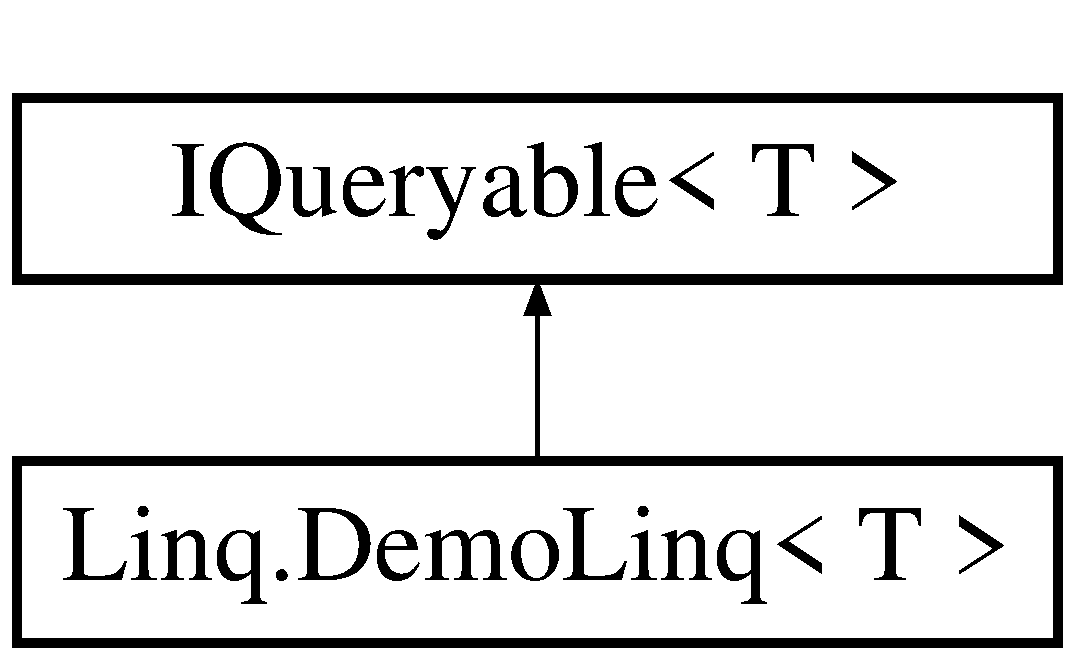
\includegraphics[height=2.000000cm]{class_linq_1_1_demo_linq}
\end{center}
\end{figure}
\subsection*{Public Member Functions}
\begin{DoxyCompactItemize}
\item 
\mbox{\Hypertarget{class_linq_1_1_demo_linq_afce055a9d9b7c32436fa552dac72613f}\label{class_linq_1_1_demo_linq_afce055a9d9b7c32436fa552dac72613f}} 
{\bfseries Demo\+Linq} (\mbox{\hyperlink{class_linq_1_1_or_mapper}{Or\+Mapper}} or\+Mapper)
\item 
\mbox{\Hypertarget{class_linq_1_1_demo_linq_a5a790bccc32e67443accd68ef09750e8}\label{class_linq_1_1_demo_linq_a5a790bccc32e67443accd68ef09750e8}} 
I\+Enumerator$<$ T $>$ {\bfseries Get\+Enumerator} ()
\end{DoxyCompactItemize}
\subsection*{Public Attributes}
\begin{DoxyCompactItemize}
\item 
\mbox{\Hypertarget{class_linq_1_1_demo_linq_a1838af085c6db0ff4702aae6adebf7fa}\label{class_linq_1_1_demo_linq_a1838af085c6db0ff4702aae6adebf7fa}} 
Type {\bfseries Element\+Type} =$>$ typeof(T)
\item 
\mbox{\Hypertarget{class_linq_1_1_demo_linq_aa3423df7efd2291f8e5a85360fb34625}\label{class_linq_1_1_demo_linq_aa3423df7efd2291f8e5a85360fb34625}} 
Expression {\bfseries Expression} =$>$ \+\_\+expression
\item 
\mbox{\Hypertarget{class_linq_1_1_demo_linq_a3efe337505d812ecd189ab8dbfcf58fc}\label{class_linq_1_1_demo_linq_a3efe337505d812ecd189ab8dbfcf58fc}} 
I\+Query\+Provider {\bfseries Provider} =$>$ \+\_\+provider
\end{DoxyCompactItemize}


The documentation for this class was generated from the following file\+:\begin{DoxyCompactItemize}
\item 
Demo\+Linq.\+cs\end{DoxyCompactItemize}

\hypertarget{class_linq_1_1_expression_tree_visitor}{}\section{Linq.\+Expression\+Tree\+Visitor Class Reference}
\label{class_linq_1_1_expression_tree_visitor}\index{Linq.\+Expression\+Tree\+Visitor@{Linq.\+Expression\+Tree\+Visitor}}
Inheritance diagram for Linq.\+Expression\+Tree\+Visitor\+:\begin{figure}[H]
\begin{center}
\leavevmode
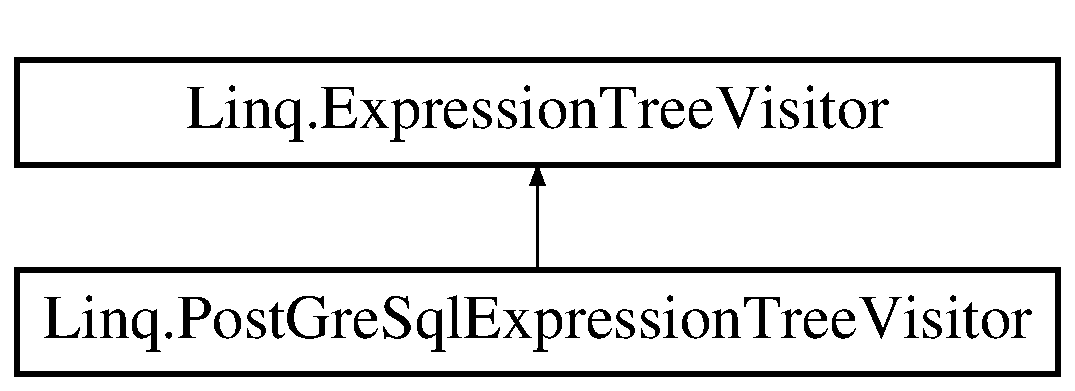
\includegraphics[height=2.000000cm]{class_linq_1_1_expression_tree_visitor}
\end{center}
\end{figure}
\subsection*{Public Member Functions}
\begin{DoxyCompactItemize}
\item 
\mbox{\Hypertarget{class_linq_1_1_expression_tree_visitor_a9a440f4c1429a26ffe410603fc0b3f34}\label{class_linq_1_1_expression_tree_visitor_a9a440f4c1429a26ffe410603fc0b3f34}} 
virtual Expression {\bfseries Visit} (Expression e)
\end{DoxyCompactItemize}
\subsection*{Protected Member Functions}
\begin{DoxyCompactItemize}
\item 
\mbox{\Hypertarget{class_linq_1_1_expression_tree_visitor_ad4182f3eb60ebd6cc5d92dd4f3387eba}\label{class_linq_1_1_expression_tree_visitor_ad4182f3eb60ebd6cc5d92dd4f3387eba}} 
virtual Member\+Binding {\bfseries Visit\+Binding} (Member\+Binding binding)
\item 
\mbox{\Hypertarget{class_linq_1_1_expression_tree_visitor_abca6f8f786bb8b81a1712577cc13360f}\label{class_linq_1_1_expression_tree_visitor_abca6f8f786bb8b81a1712577cc13360f}} 
virtual Element\+Init {\bfseries Visit\+Element\+Initializer} (Element\+Init initializer)
\item 
\mbox{\Hypertarget{class_linq_1_1_expression_tree_visitor_a535750c03443cc1272c55819f5ceed44}\label{class_linq_1_1_expression_tree_visitor_a535750c03443cc1272c55819f5ceed44}} 
virtual Expression {\bfseries Visit\+Unary} (Unary\+Expression u)
\item 
\mbox{\Hypertarget{class_linq_1_1_expression_tree_visitor_ab1a50429a5b7b0132be494e0b674cefd}\label{class_linq_1_1_expression_tree_visitor_ab1a50429a5b7b0132be494e0b674cefd}} 
virtual Expression {\bfseries Visit\+Binary} (Binary\+Expression b)
\item 
\mbox{\Hypertarget{class_linq_1_1_expression_tree_visitor_a6ab52ee5f1c1ba8829ecffb7c3269bb1}\label{class_linq_1_1_expression_tree_visitor_a6ab52ee5f1c1ba8829ecffb7c3269bb1}} 
virtual Expression {\bfseries Visit\+Type\+Is} (Type\+Binary\+Expression b)
\item 
\mbox{\Hypertarget{class_linq_1_1_expression_tree_visitor_acfd867633f6bf33f304d5ca48927418d}\label{class_linq_1_1_expression_tree_visitor_acfd867633f6bf33f304d5ca48927418d}} 
virtual Expression {\bfseries Visit\+Constant} (Constant\+Expression c)
\item 
\mbox{\Hypertarget{class_linq_1_1_expression_tree_visitor_ac167f7f6ae89b8bd98b0c8a449ee5616}\label{class_linq_1_1_expression_tree_visitor_ac167f7f6ae89b8bd98b0c8a449ee5616}} 
virtual Expression {\bfseries Visit\+Conditional} (Conditional\+Expression c)
\item 
\mbox{\Hypertarget{class_linq_1_1_expression_tree_visitor_ae92c721d152cde3879b4917e77b521e5}\label{class_linq_1_1_expression_tree_visitor_ae92c721d152cde3879b4917e77b521e5}} 
virtual Parameter\+Expression {\bfseries Visit\+Parameter} (Parameter\+Expression p)
\item 
\mbox{\Hypertarget{class_linq_1_1_expression_tree_visitor_ad911586e17f3f88f3cc191ac6f99175a}\label{class_linq_1_1_expression_tree_visitor_ad911586e17f3f88f3cc191ac6f99175a}} 
virtual Expression {\bfseries Visit\+Member\+Access} (Member\+Expression m)
\item 
\mbox{\Hypertarget{class_linq_1_1_expression_tree_visitor_a410dd70d71a8f2ef3939f4ed6a5118f7}\label{class_linq_1_1_expression_tree_visitor_a410dd70d71a8f2ef3939f4ed6a5118f7}} 
virtual Expression {\bfseries Visit\+Method\+Call} (Method\+Call\+Expression m)
\item 
\mbox{\Hypertarget{class_linq_1_1_expression_tree_visitor_a89c4c7324c509f98126b357c52a81e8e}\label{class_linq_1_1_expression_tree_visitor_a89c4c7324c509f98126b357c52a81e8e}} 
virtual Read\+Only\+Collection$<$ Expression $>$ {\bfseries Visit\+Expression\+List} (Read\+Only\+Collection$<$ Expression $>$ list)
\item 
\mbox{\Hypertarget{class_linq_1_1_expression_tree_visitor_a39b68ec5e425eb2769051aa6e30a5dac}\label{class_linq_1_1_expression_tree_visitor_a39b68ec5e425eb2769051aa6e30a5dac}} 
virtual Member\+Assignment {\bfseries Visit\+Member\+Assignment} (Member\+Assignment assignment)
\item 
\mbox{\Hypertarget{class_linq_1_1_expression_tree_visitor_af9209d068cbbe9cf9af522a1a947fcde}\label{class_linq_1_1_expression_tree_visitor_af9209d068cbbe9cf9af522a1a947fcde}} 
virtual Member\+Member\+Binding {\bfseries Visit\+Member\+Member\+Binding} (Member\+Member\+Binding binding)
\item 
\mbox{\Hypertarget{class_linq_1_1_expression_tree_visitor_a88b8c0684ccbb59dda2b3cbab53581c0}\label{class_linq_1_1_expression_tree_visitor_a88b8c0684ccbb59dda2b3cbab53581c0}} 
virtual Member\+List\+Binding {\bfseries Visit\+Member\+List\+Binding} (Member\+List\+Binding binding)
\item 
\mbox{\Hypertarget{class_linq_1_1_expression_tree_visitor_af6a665d4b5fd8ecccbc1541cad5c0d16}\label{class_linq_1_1_expression_tree_visitor_af6a665d4b5fd8ecccbc1541cad5c0d16}} 
virtual Read\+Only\+Collection$<$ Member\+Binding $>$ {\bfseries Visit\+Binding\+List} (Read\+Only\+Collection$<$ Member\+Binding $>$ list)
\item 
\mbox{\Hypertarget{class_linq_1_1_expression_tree_visitor_add7ecba789729c974b9a65d3f2aae3df}\label{class_linq_1_1_expression_tree_visitor_add7ecba789729c974b9a65d3f2aae3df}} 
virtual Read\+Only\+Collection$<$ Element\+Init $>$ {\bfseries Visit\+Element\+Initializer\+List} (Read\+Only\+Collection$<$ Element\+Init $>$ list)
\item 
\mbox{\Hypertarget{class_linq_1_1_expression_tree_visitor_a24e6f94d930b8eee5b80236fd3d91347}\label{class_linq_1_1_expression_tree_visitor_a24e6f94d930b8eee5b80236fd3d91347}} 
virtual Read\+Only\+Collection$<$ Parameter\+Expression $>$ {\bfseries Visit\+Parameter\+List} (Read\+Only\+Collection$<$ Parameter\+Expression $>$ list)
\item 
\mbox{\Hypertarget{class_linq_1_1_expression_tree_visitor_a4a173a9380f3e635fbbb5e92f71761bf}\label{class_linq_1_1_expression_tree_visitor_a4a173a9380f3e635fbbb5e92f71761bf}} 
virtual Expression {\bfseries Visit\+Lambda} (Lambda\+Expression lambda)
\item 
\mbox{\Hypertarget{class_linq_1_1_expression_tree_visitor_a1e724bcf17d06dcc4f9a6517db5dc8f9}\label{class_linq_1_1_expression_tree_visitor_a1e724bcf17d06dcc4f9a6517db5dc8f9}} 
virtual New\+Expression {\bfseries Visit\+New} (New\+Expression new\+Expression)
\item 
\mbox{\Hypertarget{class_linq_1_1_expression_tree_visitor_a1e976176e2acf4477cb002104e927ecb}\label{class_linq_1_1_expression_tree_visitor_a1e976176e2acf4477cb002104e927ecb}} 
virtual Member\+Init\+Expression {\bfseries Visit\+Member\+Init} (Member\+Init\+Expression init)
\item 
\mbox{\Hypertarget{class_linq_1_1_expression_tree_visitor_a0aaf2842a865eb9aa52014f257a5f062}\label{class_linq_1_1_expression_tree_visitor_a0aaf2842a865eb9aa52014f257a5f062}} 
virtual List\+Init\+Expression {\bfseries Visit\+List\+Init} (List\+Init\+Expression init)
\item 
\mbox{\Hypertarget{class_linq_1_1_expression_tree_visitor_a50d219d023f1268a3fa16ffab995b361}\label{class_linq_1_1_expression_tree_visitor_a50d219d023f1268a3fa16ffab995b361}} 
virtual New\+Array\+Expression {\bfseries Visit\+New\+Array} (New\+Array\+Expression na)
\item 
\mbox{\Hypertarget{class_linq_1_1_expression_tree_visitor_af65675a92ac29e1f07725385ad4c30cb}\label{class_linq_1_1_expression_tree_visitor_af65675a92ac29e1f07725385ad4c30cb}} 
virtual Expression {\bfseries Visit\+Invocation} (Invocation\+Expression iv)
\end{DoxyCompactItemize}


The documentation for this class was generated from the following file\+:\begin{DoxyCompactItemize}
\item 
Expression\+Tree\+Visitor.\+cs\end{DoxyCompactItemize}

\hypertarget{class_linq_1_1_or_mapper}{}\section{Linq.\+Or\+Mapper Class Reference}
\label{class_linq_1_1_or_mapper}\index{Linq.\+Or\+Mapper@{Linq.\+Or\+Mapper}}
\subsection*{Public Member Functions}
\begin{DoxyCompactItemize}
\item 
\mbox{\Hypertarget{class_linq_1_1_or_mapper_af7c792c7adaaa4dc9bddb28a6b76510e}\label{class_linq_1_1_or_mapper_af7c792c7adaaa4dc9bddb28a6b76510e}} 
{\bfseries Or\+Mapper} (I\+Database db, I\+Change\+Tracker ct)
\item 
I\+Queryable$<$ T $>$ \mbox{\hyperlink{class_linq_1_1_or_mapper_a61b69ea249addd0ee7c4a3e9e69022ab}{Get\+Query$<$ T $>$}} ()
\begin{DoxyCompactList}\small\item\em Gets a queryable Object (\mbox{\hyperlink{class_linq_1_1_demo_linq}{Demo\+Linq}}) \end{DoxyCompactList}\item 
I\+Enumerable$<$ T $>$ \mbox{\hyperlink{class_linq_1_1_or_mapper_a1bdf8dd049f5bbe6f4b89c22b729f4fd}{Get\+Enumerable$<$ T $>$}} (Expression expression)
\begin{DoxyCompactList}\small\item\em Executes a Select statement defined by the expression on a database and returns the results \end{DoxyCompactList}\item 
void \mbox{\hyperlink{class_linq_1_1_or_mapper_a77fcb2b43afdc48a72f6356fc063a8c2}{Insert}} (object obj)
\begin{DoxyCompactList}\small\item\em Inserts an object into the database \end{DoxyCompactList}\item 
void \mbox{\hyperlink{class_linq_1_1_or_mapper_a0a5f2100a6da15713a55ed3d972b8434}{Delete}} (object obj)
\begin{DoxyCompactList}\small\item\em Deletes an object fro the database. \end{DoxyCompactList}\item 
void \mbox{\hyperlink{class_linq_1_1_or_mapper_a447b6b90b25be80634149e945c686461}{Submit\+Changes}} ()
\begin{DoxyCompactList}\small\item\em Actually Submits the cached changes into the database all at once. \end{DoxyCompactList}\item 
bool \mbox{\hyperlink{class_linq_1_1_or_mapper_a9fb4865eedaba32daf32f65874779a60}{Is\+Type\+A\+Table}} (Type T)
\begin{DoxyCompactList}\small\item\em Checks if Type is a valid type, that can be copied to the Database \end{DoxyCompactList}\end{DoxyCompactItemize}


\subsection{Member Function Documentation}
\mbox{\Hypertarget{class_linq_1_1_or_mapper_a0a5f2100a6da15713a55ed3d972b8434}\label{class_linq_1_1_or_mapper_a0a5f2100a6da15713a55ed3d972b8434}} 
\index{Linq\+::\+Or\+Mapper@{Linq\+::\+Or\+Mapper}!Delete@{Delete}}
\index{Delete@{Delete}!Linq\+::\+Or\+Mapper@{Linq\+::\+Or\+Mapper}}
\subsubsection{\texorpdfstring{Delete()}{Delete()}}
{\footnotesize\ttfamily void Linq.\+Or\+Mapper.\+Delete (\begin{DoxyParamCaption}\item[{object}]{obj }\end{DoxyParamCaption})\hspace{0.3cm}{\ttfamily [inline]}}



Deletes an object fro the database. 


\begin{DoxyParams}{Parameters}
{\em obj} & an valid table type object that should be stored in db\\
\hline
\end{DoxyParams}
\mbox{\Hypertarget{class_linq_1_1_or_mapper_a1bdf8dd049f5bbe6f4b89c22b729f4fd}\label{class_linq_1_1_or_mapper_a1bdf8dd049f5bbe6f4b89c22b729f4fd}} 
\index{Linq\+::\+Or\+Mapper@{Linq\+::\+Or\+Mapper}!Get\+Enumerable$<$ T $>$@{Get\+Enumerable$<$ T $>$}}
\index{Get\+Enumerable$<$ T $>$@{Get\+Enumerable$<$ T $>$}!Linq\+::\+Or\+Mapper@{Linq\+::\+Or\+Mapper}}
\subsubsection{\texorpdfstring{Get\+Enumerable$<$ T $>$()}{GetEnumerable< T >()}}
{\footnotesize\ttfamily I\+Enumerable$<$T$>$ Linq.\+Or\+Mapper.\+Get\+Enumerable$<$ T $>$ (\begin{DoxyParamCaption}\item[{Expression}]{expression }\end{DoxyParamCaption})\hspace{0.3cm}{\ttfamily [inline]}}



Executes a Select statement defined by the expression on a database and returns the results 


\begin{DoxyTemplParams}{Template Parameters}
{\em T} & The Type of the table, must have Table Attribute\\
\hline
\end{DoxyTemplParams}

\begin{DoxyParams}{Parameters}
{\em expression} & A \mbox{\hyperlink{namespace_linq}{Linq}} Expression on a certain Table\\
\hline
\end{DoxyParams}
\begin{DoxyReturn}{Returns}
A List of objects of Type T 
\end{DoxyReturn}
\mbox{\Hypertarget{class_linq_1_1_or_mapper_a61b69ea249addd0ee7c4a3e9e69022ab}\label{class_linq_1_1_or_mapper_a61b69ea249addd0ee7c4a3e9e69022ab}} 
\index{Linq\+::\+Or\+Mapper@{Linq\+::\+Or\+Mapper}!Get\+Query$<$ T $>$@{Get\+Query$<$ T $>$}}
\index{Get\+Query$<$ T $>$@{Get\+Query$<$ T $>$}!Linq\+::\+Or\+Mapper@{Linq\+::\+Or\+Mapper}}
\subsubsection{\texorpdfstring{Get\+Query$<$ T $>$()}{GetQuery< T >()}}
{\footnotesize\ttfamily I\+Queryable$<$T$>$ Linq.\+Or\+Mapper.\+Get\+Query$<$ T $>$ (\begin{DoxyParamCaption}{ }\end{DoxyParamCaption})\hspace{0.3cm}{\ttfamily [inline]}}



Gets a queryable Object (\mbox{\hyperlink{class_linq_1_1_demo_linq}{Demo\+Linq}}) 


\begin{DoxyTemplParams}{Template Parameters}
{\em T} & A Table Type that is stored in the Database\\
\hline
\end{DoxyTemplParams}
\begin{DoxyReturn}{Returns}
A queryable object of Type T
\end{DoxyReturn}
\mbox{\Hypertarget{class_linq_1_1_or_mapper_a77fcb2b43afdc48a72f6356fc063a8c2}\label{class_linq_1_1_or_mapper_a77fcb2b43afdc48a72f6356fc063a8c2}} 
\index{Linq\+::\+Or\+Mapper@{Linq\+::\+Or\+Mapper}!Insert@{Insert}}
\index{Insert@{Insert}!Linq\+::\+Or\+Mapper@{Linq\+::\+Or\+Mapper}}
\subsubsection{\texorpdfstring{Insert()}{Insert()}}
{\footnotesize\ttfamily void Linq.\+Or\+Mapper.\+Insert (\begin{DoxyParamCaption}\item[{object}]{obj }\end{DoxyParamCaption})\hspace{0.3cm}{\ttfamily [inline]}}



Inserts an object into the database 


\begin{DoxyParams}{Parameters}
{\em obj} & an valid table type object that should be stored in db\\
\hline
\end{DoxyParams}
\mbox{\Hypertarget{class_linq_1_1_or_mapper_a9fb4865eedaba32daf32f65874779a60}\label{class_linq_1_1_or_mapper_a9fb4865eedaba32daf32f65874779a60}} 
\index{Linq\+::\+Or\+Mapper@{Linq\+::\+Or\+Mapper}!Is\+Type\+A\+Table@{Is\+Type\+A\+Table}}
\index{Is\+Type\+A\+Table@{Is\+Type\+A\+Table}!Linq\+::\+Or\+Mapper@{Linq\+::\+Or\+Mapper}}
\subsubsection{\texorpdfstring{Is\+Type\+A\+Table()}{IsTypeATable()}}
{\footnotesize\ttfamily bool Linq.\+Or\+Mapper.\+Is\+Type\+A\+Table (\begin{DoxyParamCaption}\item[{Type}]{T }\end{DoxyParamCaption})\hspace{0.3cm}{\ttfamily [inline]}}



Checks if Type is a valid type, that can be copied to the Database 


\begin{DoxyParams}{Parameters}
{\em T} & Type that should be checked\\
\hline
\end{DoxyParams}
\begin{DoxyReturn}{Returns}
true if Attributes are set correctly, false if there are missing or no attributes
\end{DoxyReturn}
\mbox{\Hypertarget{class_linq_1_1_or_mapper_a447b6b90b25be80634149e945c686461}\label{class_linq_1_1_or_mapper_a447b6b90b25be80634149e945c686461}} 
\index{Linq\+::\+Or\+Mapper@{Linq\+::\+Or\+Mapper}!Submit\+Changes@{Submit\+Changes}}
\index{Submit\+Changes@{Submit\+Changes}!Linq\+::\+Or\+Mapper@{Linq\+::\+Or\+Mapper}}
\subsubsection{\texorpdfstring{Submit\+Changes()}{SubmitChanges()}}
{\footnotesize\ttfamily void Linq.\+Or\+Mapper.\+Submit\+Changes (\begin{DoxyParamCaption}{ }\end{DoxyParamCaption})\hspace{0.3cm}{\ttfamily [inline]}}



Actually Submits the cached changes into the database all at once. 



The documentation for this class was generated from the following file\+:\begin{DoxyCompactItemize}
\item 
O\+R\+Mapper.\+cs\end{DoxyCompactItemize}

\hypertarget{class_linq_1_1_change_tracker_entry_1_1_pair}{}\section{Linq.\+Change\+Tracker\+Entry.\+Pair$<$ T1, T2 $>$ Class Template Reference}
\label{class_linq_1_1_change_tracker_entry_1_1_pair}\index{Linq.\+Change\+Tracker\+Entry.\+Pair$<$ T1, T2 $>$@{Linq.\+Change\+Tracker\+Entry.\+Pair$<$ T1, T2 $>$}}


Represents \mbox{\hyperlink{class_linq_1_1_change_tracker_entry_1_1_pair}{Pair}} of Values, that may be changed anytime  


\subsection*{Public Member Functions}
\begin{DoxyCompactItemize}
\item 
\mbox{\Hypertarget{class_linq_1_1_change_tracker_entry_1_1_pair_a725821fc6095b8718a129e21cf3abf56}\label{class_linq_1_1_change_tracker_entry_1_1_pair_a725821fc6095b8718a129e21cf3abf56}} 
{\bfseries Pair} (T1 item1, T2 item2)
\end{DoxyCompactItemize}
\subsection*{Properties}
\begin{DoxyCompactItemize}
\item 
\mbox{\Hypertarget{class_linq_1_1_change_tracker_entry_1_1_pair_a1ea9ce35a37cdf56f953aac814d1a805}\label{class_linq_1_1_change_tracker_entry_1_1_pair_a1ea9ce35a37cdf56f953aac814d1a805}} 
T1 {\bfseries Item1}\hspace{0.3cm}{\ttfamily  \mbox{[}get, set\mbox{]}}
\item 
\mbox{\Hypertarget{class_linq_1_1_change_tracker_entry_1_1_pair_a44b727ccb8fef8d0c26aa2f668974726}\label{class_linq_1_1_change_tracker_entry_1_1_pair_a44b727ccb8fef8d0c26aa2f668974726}} 
T2 {\bfseries Item2}\hspace{0.3cm}{\ttfamily  \mbox{[}get, set\mbox{]}}
\end{DoxyCompactItemize}


\subsection{Detailed Description}
Represents \mbox{\hyperlink{class_linq_1_1_change_tracker_entry_1_1_pair}{Pair}} of Values, that may be changed anytime 


\begin{DoxyTemplParams}{Template Parameters}
{\em T1} & \\
\hline
{\em T2} & \\
\hline
\end{DoxyTemplParams}


The documentation for this class was generated from the following file\+:\begin{DoxyCompactItemize}
\item 
Change\+Tracker\+Entry.\+cs\end{DoxyCompactItemize}

\hypertarget{class_linq_1_1_post_gre_sql_database}{}\section{Linq.\+Post\+Gre\+Sql\+Database Class Reference}
\label{class_linq_1_1_post_gre_sql_database}\index{Linq.\+Post\+Gre\+Sql\+Database@{Linq.\+Post\+Gre\+Sql\+Database}}
Inheritance diagram for Linq.\+Post\+Gre\+Sql\+Database\+:\begin{figure}[H]
\begin{center}
\leavevmode
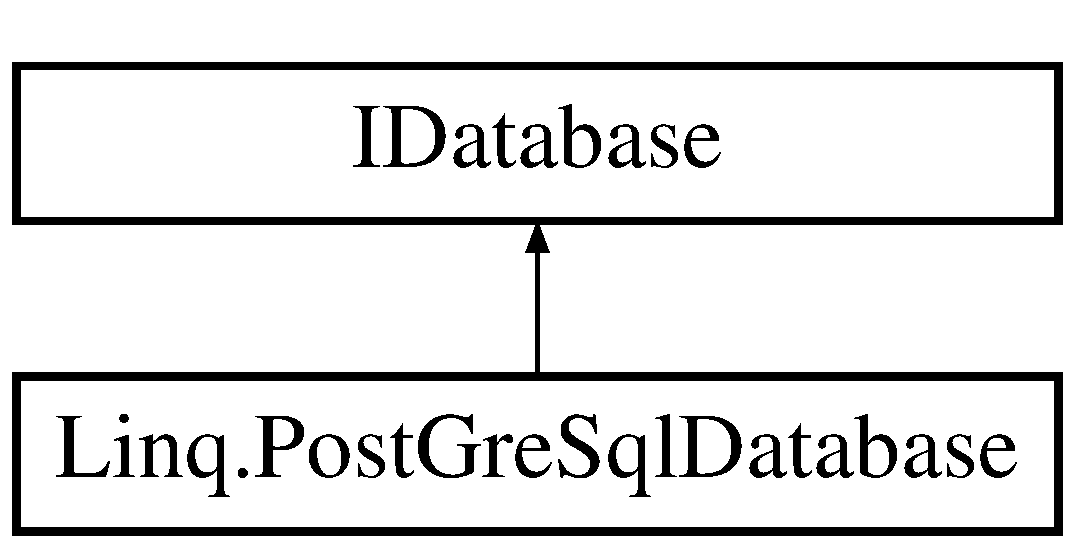
\includegraphics[height=2.000000cm]{class_linq_1_1_post_gre_sql_database}
\end{center}
\end{figure}
\subsection*{Public Member Functions}
\begin{DoxyCompactItemize}
\item 
\mbox{\Hypertarget{class_linq_1_1_post_gre_sql_database_ad038ef5510672f2e719e5d634ee48abd}\label{class_linq_1_1_post_gre_sql_database_ad038ef5510672f2e719e5d634ee48abd}} 
{\bfseries Post\+Gre\+Sql\+Database} (string connection=\char`\"{}Server=127.\+0.\+0.\+1; Port=5432; User Id=postgres; Password=postgres; Database=img\+DB\char`\"{})
\item 
\mbox{\Hypertarget{class_linq_1_1_post_gre_sql_database_a575c670d7f67ec03a9336ed3cc64cbad}\label{class_linq_1_1_post_gre_sql_database_a575c670d7f67ec03a9336ed3cc64cbad}} 
{\bfseries Post\+Gre\+Sql\+Database} (\mbox{\hyperlink{class_linq_1_1_post_gre_sql_expression_tree_visitor}{Post\+Gre\+Sql\+Expression\+Tree\+Visitor}} visitor, string connection=\char`\"{}Server=127.\+0.\+0.\+1; Port=5432; User Id=postgres; Password=postgres; Database=img\+DB\char`\"{})
\item 
I\+Enumerable$<$ T $>$ \mbox{\hyperlink{class_linq_1_1_post_gre_sql_database_abffcc78b1162e9b4b8bce35118edafca}{Select$<$ T $>$}} (Expression expression)
\begin{DoxyCompactList}\small\item\em Converts an expression into a Post\+Gre\+Sql select statement, executes it against the database and returns the Result as an enumerable \end{DoxyCompactList}\item 
int \mbox{\hyperlink{class_linq_1_1_post_gre_sql_database_ab1e6bff4c4de2da6b6173c95761929c7}{Insert$<$ T $>$}} (T new\+Object)
\begin{DoxyCompactList}\small\item\em Builds a Post\+Gre\+Sql insert statement and inserts the object into the database \end{DoxyCompactList}\item 
void \mbox{\hyperlink{class_linq_1_1_post_gre_sql_database_a61c3b22701f6aff3ca6862c2999393cb}{Delete$<$ T $>$}} (T deleted\+Object)
\begin{DoxyCompactList}\small\item\em Builds a Post\+Gre\+Sql delete statement and deletes the object from the database \end{DoxyCompactList}\item 
void \mbox{\hyperlink{class_linq_1_1_post_gre_sql_database_a8060f095f8b53fb22409a794bb41279d}{Update$<$ T $>$}} (T changed\+Object)
\begin{DoxyCompactList}\small\item\em Builds a Post\+Gre\+Sql update statement and updates the object in the database \end{DoxyCompactList}\end{DoxyCompactItemize}


\subsection{Member Function Documentation}
\mbox{\Hypertarget{class_linq_1_1_post_gre_sql_database_a61c3b22701f6aff3ca6862c2999393cb}\label{class_linq_1_1_post_gre_sql_database_a61c3b22701f6aff3ca6862c2999393cb}} 
\index{Linq\+::\+Post\+Gre\+Sql\+Database@{Linq\+::\+Post\+Gre\+Sql\+Database}!Delete$<$ T $>$@{Delete$<$ T $>$}}
\index{Delete$<$ T $>$@{Delete$<$ T $>$}!Linq\+::\+Post\+Gre\+Sql\+Database@{Linq\+::\+Post\+Gre\+Sql\+Database}}
\subsubsection{\texorpdfstring{Delete$<$ T $>$()}{Delete< T >()}}
{\footnotesize\ttfamily void Linq.\+Post\+Gre\+Sql\+Database.\+Delete$<$ T $>$ (\begin{DoxyParamCaption}\item[{T}]{deleted\+Object }\end{DoxyParamCaption})\hspace{0.3cm}{\ttfamily [inline]}}



Builds a Post\+Gre\+Sql delete statement and deletes the object from the database 


\begin{DoxyTemplParams}{Template Parameters}
{\em T} & the Table Type\\
\hline
\end{DoxyTemplParams}

\begin{DoxyParams}{Parameters}
{\em deleted\+Object} & the objects that is to be deleted\\
\hline
\end{DoxyParams}
\mbox{\Hypertarget{class_linq_1_1_post_gre_sql_database_ab1e6bff4c4de2da6b6173c95761929c7}\label{class_linq_1_1_post_gre_sql_database_ab1e6bff4c4de2da6b6173c95761929c7}} 
\index{Linq\+::\+Post\+Gre\+Sql\+Database@{Linq\+::\+Post\+Gre\+Sql\+Database}!Insert$<$ T $>$@{Insert$<$ T $>$}}
\index{Insert$<$ T $>$@{Insert$<$ T $>$}!Linq\+::\+Post\+Gre\+Sql\+Database@{Linq\+::\+Post\+Gre\+Sql\+Database}}
\subsubsection{\texorpdfstring{Insert$<$ T $>$()}{Insert< T >()}}
{\footnotesize\ttfamily int Linq.\+Post\+Gre\+Sql\+Database.\+Insert$<$ T $>$ (\begin{DoxyParamCaption}\item[{T}]{new\+Object }\end{DoxyParamCaption})\hspace{0.3cm}{\ttfamily [inline]}}



Builds a Post\+Gre\+Sql insert statement and inserts the object into the database 


\begin{DoxyTemplParams}{Template Parameters}
{\em T} & the Table Type\\
\hline
\end{DoxyTemplParams}

\begin{DoxyParams}{Parameters}
{\em new\+Object} & the objects that is to be inserted\\
\hline
\end{DoxyParams}
\begin{DoxyReturn}{Returns}
the id of the newly inserted object
\end{DoxyReturn}
\mbox{\Hypertarget{class_linq_1_1_post_gre_sql_database_abffcc78b1162e9b4b8bce35118edafca}\label{class_linq_1_1_post_gre_sql_database_abffcc78b1162e9b4b8bce35118edafca}} 
\index{Linq\+::\+Post\+Gre\+Sql\+Database@{Linq\+::\+Post\+Gre\+Sql\+Database}!Select$<$ T $>$@{Select$<$ T $>$}}
\index{Select$<$ T $>$@{Select$<$ T $>$}!Linq\+::\+Post\+Gre\+Sql\+Database@{Linq\+::\+Post\+Gre\+Sql\+Database}}
\subsubsection{\texorpdfstring{Select$<$ T $>$()}{Select< T >()}}
{\footnotesize\ttfamily I\+Enumerable$<$T$>$ Linq.\+Post\+Gre\+Sql\+Database.\+Select$<$ T $>$ (\begin{DoxyParamCaption}\item[{Expression}]{expression }\end{DoxyParamCaption})\hspace{0.3cm}{\ttfamily [inline]}}



Converts an expression into a Post\+Gre\+Sql select statement, executes it against the database and returns the Result as an enumerable 


\begin{DoxyTemplParams}{Template Parameters}
{\em T} & the Table Type\\
\hline
\end{DoxyTemplParams}

\begin{DoxyParams}{Parameters}
{\em expression} & A valid \mbox{\hyperlink{namespace_linq}{Linq}} expression without joins or complicated things\\
\hline
\end{DoxyParams}
\begin{DoxyReturn}{Returns}

\end{DoxyReturn}
\mbox{\Hypertarget{class_linq_1_1_post_gre_sql_database_a8060f095f8b53fb22409a794bb41279d}\label{class_linq_1_1_post_gre_sql_database_a8060f095f8b53fb22409a794bb41279d}} 
\index{Linq\+::\+Post\+Gre\+Sql\+Database@{Linq\+::\+Post\+Gre\+Sql\+Database}!Update$<$ T $>$@{Update$<$ T $>$}}
\index{Update$<$ T $>$@{Update$<$ T $>$}!Linq\+::\+Post\+Gre\+Sql\+Database@{Linq\+::\+Post\+Gre\+Sql\+Database}}
\subsubsection{\texorpdfstring{Update$<$ T $>$()}{Update< T >()}}
{\footnotesize\ttfamily void Linq.\+Post\+Gre\+Sql\+Database.\+Update$<$ T $>$ (\begin{DoxyParamCaption}\item[{T}]{changed\+Object }\end{DoxyParamCaption})\hspace{0.3cm}{\ttfamily [inline]}}



Builds a Post\+Gre\+Sql update statement and updates the object in the database 


\begin{DoxyTemplParams}{Template Parameters}
{\em T} & the Table Type\\
\hline
\end{DoxyTemplParams}

\begin{DoxyParams}{Parameters}
{\em changed\+Object} & the objects that is to be updated\\
\hline
\end{DoxyParams}


The documentation for this class was generated from the following file\+:\begin{DoxyCompactItemize}
\item 
Postgresql\+Database.\+cs\end{DoxyCompactItemize}

\hypertarget{class_linq_1_1_post_gre_sql_expression_tree_visitor}{}\section{Linq.\+Post\+Gre\+Sql\+Expression\+Tree\+Visitor Class Reference}
\label{class_linq_1_1_post_gre_sql_expression_tree_visitor}\index{Linq.\+Post\+Gre\+Sql\+Expression\+Tree\+Visitor@{Linq.\+Post\+Gre\+Sql\+Expression\+Tree\+Visitor}}
Inheritance diagram for Linq.\+Post\+Gre\+Sql\+Expression\+Tree\+Visitor\+:\begin{figure}[H]
\begin{center}
\leavevmode
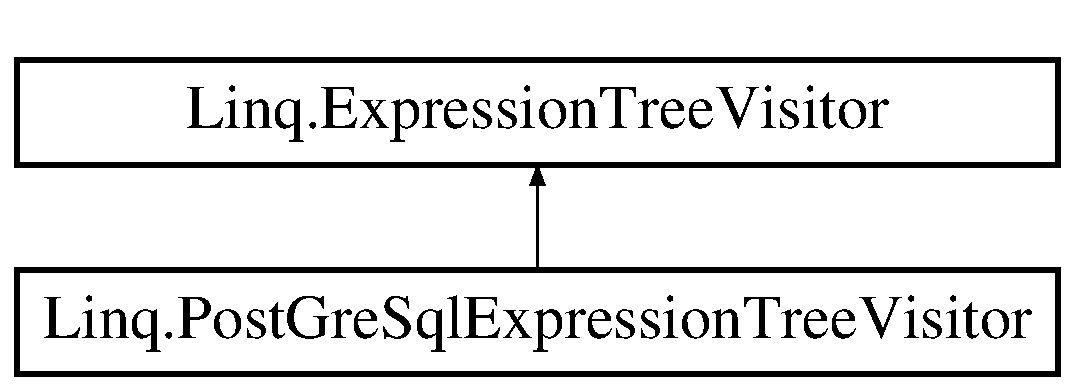
\includegraphics[height=2.000000cm]{class_linq_1_1_post_gre_sql_expression_tree_visitor}
\end{center}
\end{figure}
\subsection*{Public Member Functions}
\begin{DoxyCompactItemize}
\item 
\mbox{\Hypertarget{class_linq_1_1_post_gre_sql_expression_tree_visitor_ac89bd93ff590b05411d3637f78f4abd4}\label{class_linq_1_1_post_gre_sql_expression_tree_visitor_ac89bd93ff590b05411d3637f78f4abd4}} 
override Expression {\bfseries Visit} (Expression e)
\item 
string \mbox{\hyperlink{class_linq_1_1_post_gre_sql_expression_tree_visitor_a0f8b065e5a69ee6f610cee03f7a3fc6d}{Get\+Statement}} ()
\begin{DoxyCompactList}\small\item\em before returning the saved string the class resets its values to be ready for the next Expression \end{DoxyCompactList}\end{DoxyCompactItemize}
\subsection*{Protected Member Functions}
\begin{DoxyCompactItemize}
\item 
\mbox{\Hypertarget{class_linq_1_1_post_gre_sql_expression_tree_visitor_a6a24d5c5316fe2bd9ec99538a6fd657f}\label{class_linq_1_1_post_gre_sql_expression_tree_visitor_a6a24d5c5316fe2bd9ec99538a6fd657f}} 
override Expression {\bfseries Visit\+Method\+Call} (Method\+Call\+Expression m)
\item 
\mbox{\Hypertarget{class_linq_1_1_post_gre_sql_expression_tree_visitor_aa441c8aabe0df4cd6e6ddeed989cc633}\label{class_linq_1_1_post_gre_sql_expression_tree_visitor_aa441c8aabe0df4cd6e6ddeed989cc633}} 
override Expression {\bfseries Visit\+Lambda} (Lambda\+Expression lambda)
\item 
\mbox{\Hypertarget{class_linq_1_1_post_gre_sql_expression_tree_visitor_af65b4b608ccecbe6d5a769cf7380a911}\label{class_linq_1_1_post_gre_sql_expression_tree_visitor_af65b4b608ccecbe6d5a769cf7380a911}} 
override Expression {\bfseries Visit\+Constant} (Constant\+Expression c)
\item 
\mbox{\Hypertarget{class_linq_1_1_post_gre_sql_expression_tree_visitor_ac6fc4590508cd7cf3bf6db6f306c2db9}\label{class_linq_1_1_post_gre_sql_expression_tree_visitor_ac6fc4590508cd7cf3bf6db6f306c2db9}} 
override Parameter\+Expression {\bfseries Visit\+Parameter} (Parameter\+Expression p)
\item 
\mbox{\Hypertarget{class_linq_1_1_post_gre_sql_expression_tree_visitor_ab9a58f96730dc61df9fa0a138f9aebc9}\label{class_linq_1_1_post_gre_sql_expression_tree_visitor_ab9a58f96730dc61df9fa0a138f9aebc9}} 
override Expression {\bfseries Visit\+Member\+Access} (Member\+Expression m)
\item 
\mbox{\Hypertarget{class_linq_1_1_post_gre_sql_expression_tree_visitor_aadc30de6c3e08ef754d00bf23903e85b}\label{class_linq_1_1_post_gre_sql_expression_tree_visitor_aadc30de6c3e08ef754d00bf23903e85b}} 
override Expression {\bfseries Visit\+Binary} (Binary\+Expression b)
\end{DoxyCompactItemize}
\subsection*{Properties}
\begin{DoxyCompactItemize}
\item 
\mbox{\Hypertarget{class_linq_1_1_post_gre_sql_expression_tree_visitor_ab0296a8f9e29757e1253646102ec37f8}\label{class_linq_1_1_post_gre_sql_expression_tree_visitor_ab0296a8f9e29757e1253646102ec37f8}} 
Type {\bfseries Source\+Type}\hspace{0.3cm}{\ttfamily  \mbox{[}get\mbox{]}}
\end{DoxyCompactItemize}


\subsection{Member Function Documentation}
\mbox{\Hypertarget{class_linq_1_1_post_gre_sql_expression_tree_visitor_a0f8b065e5a69ee6f610cee03f7a3fc6d}\label{class_linq_1_1_post_gre_sql_expression_tree_visitor_a0f8b065e5a69ee6f610cee03f7a3fc6d}} 
\index{Linq\+::\+Post\+Gre\+Sql\+Expression\+Tree\+Visitor@{Linq\+::\+Post\+Gre\+Sql\+Expression\+Tree\+Visitor}!Get\+Statement@{Get\+Statement}}
\index{Get\+Statement@{Get\+Statement}!Linq\+::\+Post\+Gre\+Sql\+Expression\+Tree\+Visitor@{Linq\+::\+Post\+Gre\+Sql\+Expression\+Tree\+Visitor}}
\subsubsection{\texorpdfstring{Get\+Statement()}{GetStatement()}}
{\footnotesize\ttfamily string Linq.\+Post\+Gre\+Sql\+Expression\+Tree\+Visitor.\+Get\+Statement (\begin{DoxyParamCaption}{ }\end{DoxyParamCaption})\hspace{0.3cm}{\ttfamily [inline]}}



before returning the saved string the class resets its values to be ready for the next Expression 

\begin{DoxyReturn}{Returns}
the Where part of a Post\+Gre\+Sql select statement as a string
\end{DoxyReturn}


The documentation for this class was generated from the following file\+:\begin{DoxyCompactItemize}
\item 
Post\+Gre\+S\+Q\+L\+Expression\+Tree\+Visitor.\+cs\end{DoxyCompactItemize}

\hypertarget{class_linq_1_1_program}{}\section{Linq.\+Program Class Reference}
\label{class_linq_1_1_program}\index{Linq.\+Program@{Linq.\+Program}}


The documentation for this class was generated from the following file\+:\begin{DoxyCompactItemize}
\item 
Program.\+cs\end{DoxyCompactItemize}

%--- End generated contents ---

% Index
\backmatter
\newpage
\phantomsection
\clearemptydoublepage
\addcontentsline{toc}{chapter}{Index}
\printindex

\end{document}
